% =====================================================================
% Lösungsteil zu Kapitel 3 (Stochastik) – Lösungen zu Ü 3.1 bis Ü 3.12
% Steht am Ende des Buches hinter dem Anhang.
% Alle Ergebnisse wurden mit SymPy/SciPy nachgerechnet.
% =====================================================================
\Loesungskapitel{Lösungen zur Stochastik}

\Uebungsabschnitt{Wahrscheinlichkeitsbegriffe und bedingte Wahrscheinlichkeit}

\begin{loesung}{3.1}{Ereignisse und Axiome}
\begin{enumerate}[label=\alph*)]
  \item \[\Omega = \{1;2;3;4;5;6\},\quad A = \{2;4;6\},\quad B = \{5;6\},\quad \bar{A} = \{1;3;5\}\]
  \[A\cap B = \{6\},\qquad A\cup B = \{2;4;5;6\}\]
  \item Laplace-Experiment: $P(E) = \dfrac{|E|}{|\Omega|}$.
  \[P(A\cap B) = \dfrac{1}{6},\qquad P(A\cup B) = \dfrac{4}{6} = \dfrac{2}{3}\]
  \textit{Kontrolle} mit dem Additionssatz: $P(A)+P(B)-P(A\cap B) = \frac{3}{6}+\frac{2}{6}-\frac{1}{6} = \frac{4}{6}$.
  \item Unvereinbar heißt $A\cap B = \{\}$. Hier ist $A\cap B = \{6\}\neq\{\}$: Bei der Augenzahl $6$ treten beide Ereignisse gleichzeitig ein. $A$ und $B$ sind also \textbf{nicht} unvereinbar.
  \item Für jedes Ereignis $E$ gilt $E\cup\bar{E} = \Omega$ und $E\cap\bar{E} = \{\}$, die beiden Ereignisse sind also unvereinbar.
  \begin{align*}
    1 &= P(\Omega) && \text{(Normierung)}\\
      &= P(E\cup\bar{E}) = P(E)+P(\bar{E}) && \text{(Additivität, da $E$, $\bar{E}$ unvereinbar)}
  \end{align*}
  Umstellen ergibt $P(\bar{E}) = 1-P(E)$.
\end{enumerate}
\end{loesung}

\begin{loesung}{3.2}{Bedingte Wahrscheinlichkeit}
\begin{enumerate}[label=\alph*)]
  \item Die erste Stufe gibt an, ob die Person erkrankt ist, die zweite das Testergebnis. An den Ästen der zweiten Stufe stehen bedingte Wahrscheinlichkeiten, an den Pfadenden die Pfadwahrscheinlichkeiten (Produkt entlang des Pfades, 1.~Pfadregel).
  \begin{center}
  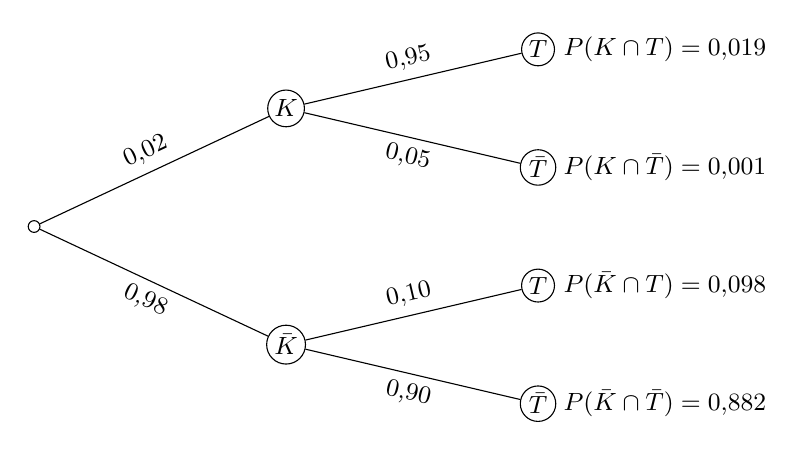
\begin{tikzpicture}[grow=right, sloped,
      level 1/.style={level distance=3.2cm, sibling distance=3cm},
      level 2/.style={level distance=3.2cm, sibling distance=1.5cm},
      every node/.style={font=\small}]
    \node[circle, draw, inner sep=1.5pt] {}
      child {node[circle, draw, inner sep=1pt] {$\bar{K}$}
        child {node[circle, draw, inner sep=1pt] (a) {$\bar{T}$}
          edge from parent node[below] {$0{,}90$}}
        child {node[circle, draw, inner sep=1pt] (b) {$T$}
          edge from parent node[above] {$0{,}10$}}
        edge from parent node[below] {$0{,}98$}}
      child {node[circle, draw, inner sep=1pt] {$K$}
        child {node[circle, draw, inner sep=1pt] (c) {$\bar{T}$}
          edge from parent node[below] {$0{,}05$}}
        child {node[circle, draw, inner sep=1pt] (d) {$T$}
          edge from parent node[above] {$0{,}95$}}
        edge from parent node[above] {$0{,}02$}};
    \node[right=2mm] at (d) {$P(K\cap T) = 0{,}019$};
    \node[right=2mm] at (c) {$P(K\cap\bar{T}) = 0{,}001$};
    \node[right=2mm] at (b) {$P(\bar{K}\cap T) = 0{,}098$};
    \node[right=2mm] at (a) {$P(\bar{K}\cap\bar{T}) = 0{,}882$};
  \end{tikzpicture}
  \end{center}
  \item 2.~Pfadregel (Summe der Pfade, die zu $T$ führen):
  \[P(T) = 0{,}02\cdot 0{,}95+0{,}98\cdot 0{,}10 = 0{,}019+0{,}098 = 0{,}117\]
  \item Definition der bedingten Wahrscheinlichkeit:
  \[P_T(K) = \dfrac{P(T\cap K)}{P(T)} = \dfrac{0{,}019}{0{,}117}\approx 0{,}1624\]
  \textit{Interpretation:} Von allen Personen mit positivem Test sind nur etwa $16\,\%$ tatsächlich erkrankt.
  \item Ein positives Testergebnis hat nur eine geringe Aussagekraft. Etwa $84\,\%$ der positiven Ergebnisse sind falsch positiv. Der Grund ist die geringe Verbreitung der Krankheit: Die Gesunden sind so zahlreich, dass schon $10\,\%$ falsch positive Ergebnisse ($0{,}098$) deutlich mehr ausmachen als die richtig positiven ($0{,}019$). Immerhin steigt die Wahrscheinlichkeit, erkrankt zu sein, durch den positiven Test von $2\,\%$ auf etwa $16\,\%$. Ein positives Ergebnis sollte deshalb durch einen genaueren Test überprüft werden. Ein negatives Ergebnis ist dagegen sehr verlässlich: $P_{\bar{T}}(\bar{K}) = \frac{0{,}882}{0{,}883}\approx 0{,}9989$.
\end{enumerate}
\end{loesung}

\Uebungsabschnitt{Zufallsgrößen, Erwartungswert und Varianz}

\begin{loesung}{3.3}{Glücksrad}
\begin{enumerate}[label=\alph*)]
  \item Gewinn $=$ Auszahlung $-$ Einsatz:
  \begin{center}\begin{tabular}{|c|c|c|c|}
    \hline
    $x_i$ (in €) & $0-1 = -1$ & $1-1 = 0$ & $4-1 = 3$\\
    \hline
    $P(X=x_i)$ & $\frac{1}{2}$ & $\frac{1}{3}$ & $\frac{1}{6}$\\
    \hline
  \end{tabular}\end{center}
  \item Ein Spiel ist fair, wenn der Erwartungswert des Gewinns $0$ ist.
  \[E(X) = (-1)\cdot\dfrac{1}{2}+0\cdot\dfrac{1}{3}+3\cdot\dfrac{1}{6} = -\dfrac{1}{2}+\dfrac{1}{2} = 0\]
  \item Definition der Varianz mit $\mu=0$:
  \[Var(X) = (-1-0)^2\cdot\dfrac{1}{2}+(0-0)^2\cdot\dfrac{1}{3}+(3-0)^2\cdot\dfrac{1}{6} = \dfrac{1}{2}+0+\dfrac{3}{2} = 2\]
  \[\sigma = \sqrt{Var(X)} = \sqrt{2}\approx 1{,}41\ \text{€}\]
  \item $F(0) = P(X\leq 0) = P(X=-1)+P(X=0) = \dfrac{1}{2}+\dfrac{1}{3} = \dfrac{5}{6}$
  \item Der Betreiber nimmt im Mittel $0{,}25$\,€ ein, wenn der Spieler im Mittel $0{,}25$\,€ verliert, also $E(X) = -0{,}25$. Mit dem neuen Betrag $a$ (in €) ist der Gewinn in diesem Sektor $a-1$:
  \[(-1)\cdot\dfrac{1}{2}+0\cdot\dfrac{1}{3}+(a-1)\cdot\dfrac{1}{6} = -\dfrac{1}{4}\quad\Longleftrightarrow\quad\dfrac{a-1}{6} = \dfrac{1}{4}\quad\Longleftrightarrow\quad a = 2{,}5\]
  Im Sektor \glqq 4\,€\grqq{} dürfen nur noch $2{,}50$\,€ ausgezahlt werden.
\end{enumerate}
\end{loesung}
\newpage
\Uebungsabschnitt{Kombinatorik und hypergeometrische Verteilung}

\begin{loesung}{3.4}{Kombinatorik}
\textit{Grundlage:} Übersichtstabelle der Kombinatorik (Ziehen mit oder ohne Zurücklegen, mit oder ohne Beachtung der Reihenfolge).
\begin{enumerate}[label=\alph*)]
  \item Reihenfolge wichtig, Ziffern dürfen sich wiederholen (\glqq mit Zurücklegen\grqq), $n=10$, $k=4$:\quad $10^4 = 10\,000$
  \item Reihenfolge wichtig, ohne Wiederholung:\quad $\dfrac{10!}{6!} = 10\cdot 9\cdot 8\cdot 7 = 5040$
  \item Alle Anordnungen von $5$ verschiedenen Objekten (Permutationen):\quad $5! = 120$
  \item Reihenfolge unwichtig, ohne Wiederholung:\quad $\dbinom{5}{2} = \dfrac{5\cdot 4}{2\cdot 1} = 10$
  \item Reihenfolge unwichtig, ohne Zurücklegen:\quad $\dbinom{49}{6}$\quad (Wert zur Information: $13\,983\,816$)
\end{enumerate}
\end{loesung}

\begin{loesung}{3.5}{Hypergeometrische Verteilung}
\begin{enumerate}[label=\alph*)]
  \item Die Grundgesamtheit besteht aus zwei Sorten von Objekten ($4$ defekte, $16$ intakte Glühbirnen). Es werden $5$ Stück auf einmal, also ohne Zurücklegen und ohne Beachtung der Reihenfolge, gezogen, und $X$ zählt die Objekte einer Sorte. Das ist genau das Urnenmodell der hypergeometrischen Verteilung. Eine Binomialverteilung liegt nicht vor, weil sich die Wahrscheinlichkeit für \glqq defekt\grqq{} nach jeder Entnahme ändert.
  \item Hypergeometrische Wahrscheinlichkeit, $\frac{\text{günstige}}{\text{mögliche}}$ Auswahlen:
  \[P(X=1) = \dfrac{\binom{4}{1}\cdot\binom{16}{4}}{\binom{20}{5}} = \dfrac{4\cdot 1820}{15\,504} = \dfrac{7280}{15\,504}\approx 0{,}4696\]
  \item Gegenereignis \glqq keine defekte Glühbirne\grqq:
  \[P(X\geq 1) = 1-P(X=0) = 1-\dfrac{\binom{4}{0}\cdot\binom{16}{5}}{\binom{20}{5}} = 1-\dfrac{4368}{15\,504}\approx 1-0{,}2817 = 0{,}7183\]
\end{enumerate}
\end{loesung}

\Uebungsabschnitt{Bernoulli-Kette und Binomialverteilung}

\begin{loesung}{3.6}{Multiple-Choice-Test}
\begin{enumerate}[label=\alph*)]
  \item Jede Frage ist ein Bernoulli-Experiment mit \glqq richtig\grqq{} (Treffer) und \glqq falsch\grqq. Wegen des zufälligen Ankreuzens ist die Trefferwahrscheinlichkeit bei jeder Frage $p=\frac{1}{4}$, und die Fragen werden unabhängig voneinander beantwortet. Damit liegt eine Bernoulli-Kette der Länge $10$ vor, und $X$ ist nach $B(10;0{,}25)$ verteilt.
  \item Bernoulli-Formel bzw. kumulative Verteilungsfunktion (Werte mit dem Rechner):
  \begin{align*}
    P(A) &= P^{10}_{0{,}25}(X=3) = \dbinom{10}{3}\cdot 0{,}25^3\cdot 0{,}75^7\approx 0{,}2503\\
    P(B) &= P^{10}_{0{,}25}(X\leq 2)\approx 0{,}5256\\
    P(C) &= P^{10}_{0{,}25}(X\geq 5) = 1-P^{10}_{0{,}25}(X\leq 4)\approx 1-0{,}92187 = 0{,}0781\\
    P(D) &= P^{10}_{0{,}25}(2\leq X\leq 4) = P^{10}_{0{,}25}(X\leq 4)-P^{10}_{0{,}25}(X\leq 1)\\
         &\approx 0{,}92187-0{,}24403\approx 0{,}6778
  \end{align*}
  \item Erwartungswert und Varianz der Binomialverteilung:
  \[E(X) = n\cdot p = 10\cdot 0{,}25 = 2{,}5,\qquad\sigma = \sqrt{n\cdot p\cdot(1-p)} = \sqrt{1{,}875}\approx 1{,}37\]
  Vergleich der Einzelwahrscheinlichkeiten in der Nähe von $\mu$:
  \[P(X=1)\approx 0{,}1877,\quad P(X=2)\approx 0{,}2816,\quad P(X=3)\approx 0{,}2503\]
  Am wahrscheinlichsten sind $2$ richtige Antworten. (Für weiter entfernte Werte werden die Wahrscheinlichkeiten noch kleiner.)
\end{enumerate}
\end{loesung}

\begin{loesung}{3.7}{3-m-Aufgaben}
\textit{Verfahren:} \glqq mindestens ein Treffer\grqq{} über das Gegenereignis \glqq kein Treffer\grqq, $P(X\geq 1) = 1-(1-p)^n$.
\begin{enumerate}[label=\alph*)]
  \item \begin{align*}
    1-0{,}95^n &\geq 0{,}95\\
    0{,}95^n &\leq 0{,}05 \quad\big|\,\ln\\
    n\cdot\ln{(0{,}95)} &\leq \ln{(0{,}05)} \quad\big|\,:\ln{(0{,}95)}<0 \text{ (Ungleichheitszeichen dreht sich um)}\\
    n &\geq \dfrac{\ln{(0{,}05)}}{\ln{(0{,}95)}}\approx 58{,}4
  \end{align*}
  Man muss mindestens $59$ Bauteile prüfen.\\
  \textit{Kontrolle:} $1-0{,}95^{58}\approx 0{,}9490 < 0{,}95$, aber $1-0{,}95^{59}\approx 0{,}9515\geq 0{,}95$.
  \item \begin{align*}
    1-(1-p)^{20} &\geq 0{,}9\\
    (1-p)^{20} &\leq 0{,}1\\
    1-p &\leq 0{,}1^{\frac{1}{20}}\approx 0{,}89125\\
    p &\geq 1-0{,}1^{\frac{1}{20}}\approx 0{,}10875
  \end{align*}
  Die Trefferwahrscheinlichkeit muss mindestens etwa $0{,}1088$ betragen, also rund $10{,}9\,\%$. (Wegen \glqq mindestens\grqq{} wird aufgerundet: Mit $p=0{,}1087$ ergibt sich nur $0{,}89989 < 0{,}9$.)
\end{enumerate}
\end{loesung}

\begin{loesung}{3.8}{\texorpdfstring{\(\sigma\)}{Sigma}-Umgebung}
\begin{enumerate}[label=\alph*)]
  \item \[\mu = n\cdot p = 100\cdot 0{,}3 = 30,\qquad\sigma = \sqrt{100\cdot 0{,}3\cdot 0{,}7} = \sqrt{21}\approx 4{,}58\]
  \item \[[\mu-2\sigma;\mu+2\sigma]\approx[30-9{,}17;30+9{,}17] = [20{,}83;39{,}17]\]
  Ganzzahlige Werte in der Umgebung: $21;22;\ldots;39$.
  \item \[P(21\leq X\leq 39) = P^{100}_{0{,}3}(X\leq 39)-P^{100}_{0{,}3}(X\leq 20)\approx 0{,}9790-0{,}0165 = 0{,}9625\]
  (Das passt zur Faustregel, nach der in der $2\sigma$-Umgebung etwa $95\,\%$ der Werte liegen.)
  \item $45$ liegt weit außerhalb der $2\sigma$-Umgebung und sogar außerhalb der $3\sigma$-Umgebung ($\mu+3\sigma\approx 43{,}7$).
  \[P^{100}_{0{,}3}(X\geq 45) = 1-P^{100}_{0{,}3}(X\leq 44)\approx 0{,}0011\]
  Ein so großes Ergebnis ist unter der Annahme $p=0{,}3$ äußerst unwahrscheinlich (etwa $1$ zu $900$). Es spricht dafür, dass die Trefferwahrscheinlichkeit größer als $0{,}3$ ist. Beweisen lässt sich das mit einem einzigen Ergebnis aber nicht.
\end{enumerate}
\end{loesung}

\Uebungsabschnitt{Hypothesentest}

\begin{loesung}{3.9}{Fehler beim Testen}
Testgröße $X$: Anzahl defekter Bauteile unter $50$, nach $B(50;p)$ verteilt.
\begin{enumerate}[label=\alph*)]
  \item $K = \{9;10;\ldots;50\}$ (Ablehnungsbereich), $\bar{K} = \{0;1;\ldots;8\}$ (Annahmebereich).
  \item \textit{Fehler erster Art:} Der Abnehmer lehnt die Behauptung des Herstellers ab (mindestens $9$ defekte Bauteile in der Stichprobe), obwohl tatsächlich höchstens $10\,\%$ der Bauteile defekt sind.\\
  \textit{Fehler zweiter Art:} Der Abnehmer behält die Behauptung bei (höchstens $8$ defekte Bauteile in der Stichprobe), obwohl tatsächlich mehr als $10\,\%$ der Bauteile defekt sind.
  \item \[\alpha = P^{50}_{0{,}1}(X\geq 9) = 1-P^{50}_{0{,}1}(X\leq 8)\approx 1-0{,}9421 = 0{,}0579\]
  \item \[\beta = P^{50}_{0{,}2}(X\leq 8)\approx 0{,}3073\]
  \item Gesucht ist das kleinste $k$ mit $P^{50}_{0{,}1}(X\geq k)\leq 0{,}05$, also mit $P^{50}_{0{,}1}(X\leq k-1)\geq 0{,}95$.
  \begin{center}\begin{tabular}{|c|c|c|}
    \hline
    $k$ & $P^{50}_{0{,}1}(X\leq k-1)$ & $P^{50}_{0{,}1}(X\geq k)$\\
    \hline
    $9$ & $0{,}9421$ & $0{,}0579 > 0{,}05$\\
    \hline
    $10$ & $0{,}9755$ & $0{,}0245\leq 0{,}05$\\
    \hline
  \end{tabular}\end{center}
  Der kleinste Wert ist $k=10$, also $K = \{10;11;\ldots;50\}$.
  \item Der Ablehnungsbereich wird kleiner und der Annahmebereich größer ($\bar{K} = \{0;\ldots;9\}$). Die Wahrscheinlichkeit für den Fehler zweiter Art steigt deshalb, z.\,B. für $p=0{,}2$:
  \[\beta = P^{50}_{0{,}2}(X\leq 9)\approx 0{,}4437 > 0{,}3073\]
  Durch eine Änderung der Entscheidungsregel lässt sich eine Fehlerwahrscheinlichkeit nur auf Kosten der anderen verringern. Beide zugleich verringert man, indem man den \textbf{Stichprobenumfang} erhöht, also mehr Bauteile prüft. Das ist allerdings mit höheren Kosten verbunden.
\end{enumerate}
\end{loesung}

\Uebungsabschnitt{Stetige Zufallsgrößen und Normalverteilung}

\begin{loesung}{3.10}{Dichtefunktion}
\begin{enumerate}[label=\alph*)]
  \item Eine Dichtefunktion ist nicht negativ, und die Gesamtfläche unter ihrem Graphen ist $1$. Für $k>0$ und $0\leq x\leq 4$ ist $k\cdot x\cdot(4-x)\geq 0$. Normierung:
  \[\integral[limits-mode=limits,limits={0, 4}]{k\cdot(4x-x^2)} = k\cdot\left[2x^2-\dfrac{1}{3}x^3\right]_0^4 = k\cdot\left(32-\dfrac{64}{3}\right) = \dfrac{32}{3}k = 1\quad\Longrightarrow\quad k = \dfrac{3}{32}\]
  \item \begin{align*}
    P(1\leq X\leq 3) &= \dfrac{3}{32}\left[2x^2-\dfrac{1}{3}x^3\right]_1^3 = \dfrac{3}{32}\left((18-9)-\left(2-\dfrac{1}{3}\right)\right)\\
    &= \dfrac{3}{32}\cdot\dfrac{22}{3} = \dfrac{11}{16} = 0{,}6875
  \end{align*}
  \item $G_f$ ist über $[0;4]$ eine nach unten geöffnete Parabel mit den Nullstellen $0$ und $4$. Sie ist achsensymmetrisch zur Geraden $x=2$, d.\,h. $f(2-t) = f(2+t)$. Die Wahrscheinlichkeitsmasse verteilt sich also symmetrisch um $2$, und der Erwartungswert als \glqq Schwerpunkt\grqq{} liegt bei $E(X)=2$.
  \item Definition der Varianz einer stetigen Zufallsgröße mit $\mu=2$. Zunächst ausmultiplizieren:
  \[(x-2)^2\cdot x(4-x) = (x^2-4x+4)(4x-x^2) = -x^4+8x^3-20x^2+16x\]
  \begin{align*}
    Var(X) &= \dfrac{3}{32}\integral[limits-mode=limits,limits={0, 4}]{\left(-x^4+8x^3-20x^2+16x\right)} = \dfrac{3}{32}\left[-\dfrac{1}{5}x^5+2x^4-\dfrac{20}{3}x^3+8x^2\right]_0^4\\
    &= \dfrac{3}{32}\left(-\dfrac{1024}{5}+512-\dfrac{1280}{3}+128\right) = \dfrac{3}{32}\cdot\dfrac{128}{15} = \dfrac{4}{5} = 0{,}8
  \end{align*}
  ($\sigma = \sqrt{0{,}8}\approx 0{,}89$)
  \item $P(X=2) = \integral[limits-mode=limits,limits={2, 2}]{f(x)} = 0$. Bei einer stetigen Zufallsgröße ist die Wahrscheinlichkeit für einen einzelnen Wert stets $0$, denn über einem Intervall der Breite $0$ gibt es keine Fläche. Positive Wahrscheinlichkeiten haben nur Intervalle.
\end{enumerate}
\end{loesung}

\begin{loesung}{3.11}{Gauß'sche Glockenkurve}
\begin{enumerate}[label=\alph*)]
  \item Kettenregel, dann Produktregel (der Faktor $\frac{1}{\sqrt{2\pi}}$ bleibt erhalten):
  \begin{align*}
    \varphi_{0;1}'(x) &= \dfrac{1}{\sqrt{2\pi}}\cdot(-x)\cdot e^{-\frac{x^2}{2}}\\
    \varphi_{0;1}''(x) &= \dfrac{1}{\sqrt{2\pi}}\left[(-1)\cdot e^{-\frac{x^2}{2}}+(-x)\cdot(-x)\cdot e^{-\frac{x^2}{2}}\right] = \dfrac{1}{\sqrt{2\pi}}\cdot(x^2-1)\cdot e^{-\frac{x^2}{2}}
  \end{align*}
  Weil $\frac{1}{\sqrt{2\pi}}e^{-\frac{x^2}{2}}>0$ ist, gilt $\varphi_{0;1}''(x)=0\Longleftrightarrow x^2-1=0\Longleftrightarrow x=\pm 1$. Der Faktor $x^2-1$ hat bei $\pm 1$ einfache Nullstellen und wechselt dort das Vorzeichen. Der Graph besitzt also bei $x=-1$ und $x=1$ Wendepunkte.
  \item Der Hochpunkt der Glockenkurve liegt bei $x=\mu$, also $\mu = 10$. Der Hochwert ist $\varphi_{\mu;\sigma}(\mu) = \dfrac{1}{\sigma\sqrt{2\pi}}$:
  \[\dfrac{1}{\sigma\sqrt{2\pi}} = 0{,}2\quad\Longleftrightarrow\quad\sigma = \dfrac{1}{0{,}2\cdot\sqrt{2\pi}}\approx 1{,}995\approx 2{,}0\]
  Die Wendestellen liegen bei $\mu\pm\sigma$, also bei $x\approx 8$ und $x\approx 12$ (genauer $8{,}005$ und $11{,}995$).
  \item Bei Verdopplung von $\sigma$
  \begin{itemize}
    \item wird der Graph in Richtung der $x$-Achse um $\mu$ mit dem Faktor $2$ gestreckt (er wird breiter, die Wendestellen rücken von $\mu\pm\sigma$ nach $\mu\pm 2\sigma$),
    \item halbiert sich der Hochwert $\frac{1}{\sigma\sqrt{2\pi}}$ (die Kurve wird flacher),
    \item bleibt die Symmetrieachse $x=\mu$ und die Gesamtfläche $1$ unverändert.
  \end{itemize}
\end{enumerate}
\end{loesung}

\begin{loesung}{3.12}{Normalverteilung und \texorpdfstring{\(\sigma\)}{Sigma}-Regeln}
$\mu = 500$, $\sigma = 4$.
\begin{enumerate}[label=\alph*)]
  \item $492 = 500-2\cdot 4 = \mu-2\sigma$. Nach den $\sigma$-Regeln gilt $P(\mu-2\sigma\leq X\leq\mu+2\sigma)\approx 0{,}954$. Der Rest $0{,}046$ verteilt sich wegen der Symmetrie der Glockenkurve gleichmäßig auf beide Seiten:
  \[P(X<492)\approx\dfrac{1-0{,}954}{2} = 0{,}023\]
  \item \[P(495\leq X\leq 505) = \Phi_{500;4}(505)-\Phi_{500;4}(495)\approx 0{,}89435-0{,}10565\approx 0{,}7887\]
  \item $\sigma$-Regel $P(\mu-1{,}96\sigma\leq X\leq\mu+1{,}96\sigma)\approx 0{,}950$ mit $1{,}96\cdot 4 = 7{,}84$:
  \[I = [500-7{,}84;500+7{,}84] = [492{,}16;507{,}84]\]
  \item Exakter Wert: $p = P(X<492) = \Phi_{500;4}(492)\approx 0{,}02275$.\\
  Die $20$ Flaschen werden unabhängig voneinander ausgewählt. Die Anzahl $Y$ der Flaschen unter $492$\,ml ist also nach $B(20;p)$ verteilt. Über das Gegenereignis:
  \[P(Y\geq 1) = 1-(1-p)^{20}\approx 1-0{,}97725^{20}\approx 0{,}3689\]
  \item \textit{Für das Modell spricht:} Die Füllmenge ist eine stetige Größe. Sie streut durch viele kleine, voneinander unabhängige Einflüsse (Maschine, Druck, Temperatur) symmetrisch um den Sollwert. Abweichungen in beide Richtungen sind gleich wahrscheinlich, große Abweichungen selten.\\
  \textit{Einschränkungen:} Die Normalverteilung ordnet auch unmöglichen Werten (z.\,B. negativen Füllmengen oder Mengen über dem Flascheninhalt) eine positive Wahrscheinlichkeit zu. Diese ist bei $\sigma=4$\,ml aber verschwindend klein. Ob die Werte in der Realität tatsächlich symmetrisch streuen, müsste man an Messdaten prüfen (z.\,B. könnten unterfüllte Flaschen aussortiert werden). Insgesamt ist die Modellierung sinnvoll.
\end{enumerate}
\end{loesung}

\LoesungskapitelEnde
